% Set the author and title of the compiled pdf
\hypersetup{
  pdftitle = {\Title},
  pdfauthor = {\Author}
}

\section{Finite precision computation}

Unfortunately, the world is not solely restricted to integers, and computers
often need to work with real numbers $\mathbb{R}$. With integers, the main
problem we have in computer terms is overflow, and since there is a finite
distance from one to the next, they are easy to encode in a computer.

On the other hand, between any two real numbers, there are infinitely many more
real numbers. Since computers are discrete, we need to sample the real numbers
so that we can find a representation for them in the computer. However, this
introduces errors, since we can't represent every value exactly and therefore
most approximate.

\subsection{Floating point numbers}

%Slide 1

One problem we have with computation is that we don't know what the error is
with computations; how `good' is the result of an algorithm or computation? We
would like to know the error bounds of a solution, and have the output be
reliable.

%Slide 2

In the $70$'s, it was realised that different floating point implementations
produced different results. This had significant concerns for reproducability,
and as a result the ANSII IEEE standard for binary floating point arithmetic was
created.

%Slide 3

Each floating point number is represented as four integers; the base, the
precision, the exponent and the mantissa.

\[
  x = \pm m \times b^{e-n}
\]

Where:

\begin{center}
  \begin{tabular}{>{$}l<{$}|l}
    m & The Mantissa (the bit before the decimal place)\\
    b & The base (or radix), usually two or ten\\
    e & The exponent (the power of the radix)\\
    n & The precision (the number of digits in the mantissa)
  \end{tabular}
\end{center}

We can represent different numbers in different ways, for example:

\[
  0.121e10^3 = 0.0121e10^4
\]

In this case, we can normalise the way in which we represent numbers and at
least all computers will get the same errors.

% Slide 4

The amount of numbers we can represent with the floating points depends on the
values permissible for $b,n$ and $e$. When $b=2,n=2$ and $e=[-2\dots2]$:

\marginpar{The Python code used to generate this is found in the
\texttt{/COMP36212/programs} folder of the source for these notes.}

\begin{center}
  \begin{tabular}{>{$}c<{$} >{$}c<{$} >{$}c<{$} >{$}c<{$} >{$}c<{$}}
    2 & \times & 2^{-2} & = & 0.500000\\
    3 & \times & 2^{-2} & = & 0.750000\\
    2 & \times & 2^{-1} & = & 1.000000\\
    3 & \times & 2^{-1} & = & 1.500000\\
    2 & \times & 2^{0} & = & 2.000000\\
    3 & \times & 2^{0} & = & 3.000000\\
    2 & \times & 2^{1} & = & 4.000000\\
    3 & \times & 2^{1} & = & 6.000000\\
    2 & \times & 2^{2} & = & 8.000000\\
    3 & \times & 2^{2} & = & 12.000000\\
  \end{tabular}
\end{center}

The mantissa is always $2$ or $3$ since we're using an explicit one, so the
binary values are either $[1,0]$ or $[1,1]$.

Floating point numbers are relatively spaced; even though they might not be the
same distance apart, the ratio between them is the same. The unit round off
(basically the last digit) is called the \textit{relative machine precision}.

The \textbf{Relative Machine Precision} is given by $u = 0.5 \times b^{1 - n}$,
and is the largest possible difference between a real number and its floating
point representation. In the above example, $u = 0.5 \times 2^{-1} =
\frac{1}{4}$. The value $2u$ is called the \textbf{Machine Precision}.

%Slide 5

In the exam, assume explicit storage of leading bit of mantissa.

\subsubsection{Real world floats}

% TODO: Insert diagram of float format here

For the sign bit, $0$ is for positive numbers and $1$ is for negative ones. The
exponent must also be able to represent negative numbers (in the case of
$24\times2^{-2}$ for example), and thus in single precision floats, a bias of
$+127$ is added to the exponent and that value is stored. The exponent values
$-127$ and $+128$ are reserved for special numbers.

The first bit of the mantissa is implicitly $1$ in the IEEE base two floating
point representation. This is because normalised numbers always have $1$ as the
first digit of their mantissa, and then we can get another digit of precision.

% TODO: Ranges of floating point numbers slide 1

Sixty-four bit floating point numbers have one sign bit, $11$ exponent bits and
$52$ mantissa bits. This means their bias will be $2^{11} = 2048$ and the range
will be $2 - 2^{52} \times 2^{2^{11}}$.

The standard also has special values built in:

\begin{description}
  \item \textbf{Zero}: When the exponent is all zeros and the mantissa equal to 
  zero.
  \item \textbf{Denormalised number}: If the exponent is all zero, but the
  mantissa is non-zero, then the number is
  $-1^{sign} \times 0.m\times 2^{-126}$.
  \item \textbf{Infinity}: Exponent is all 1's and mantissa is all 0's. The
  sign dictates between positive and negative infinity.
  %TODO: Signalling and quite NaN's
  \item \textbf{NaN}: Not your grandma, this is when the value isn't a real
  number, such as when a division by zero occurs.The exponent is all 1's and
  the mantissa is non-zero.
\end{description}

\subsubsection{Error in floating point numbers}
% Example exam q:
% Given a decimal number x, convert it to normal form and then into binary
% with specific values for e, m and b. Then trunctuate/round it and estimate
% the error

% TODO: How can a computer work out this error? It only knows floats...

When a real number is converted to floating point number, it may lose precision.
If the real number if $x$ and the floating point representation is
$\bar{x}$, then the error is:

\[
  e = \bar{x} - x
\]

You can find how many significant digits a floating point number approximates a
real number to by doing:

\[
  |\bar{x} - x| = 10^{-\text{significant digits}}
\]


However, the absolute error $e$ does not give us a good description of the
accuracy (if the error is $10^{-6}$ but the value is $10^{-7}$ then we're very,
very inaccurate)! To rectify this, we have relative error:

\[
  r = \frac{e}{x} = \frac{\bar{x} - x}{x}
\]

%TODO: Wat is bounds?!

When we're getting the floating point number from the real number, we can
truncate the (possibly infinite) digits so that it fits in the mantissa. Simply
chopping the number so it fits in $m$ bits is called \textbf{simple truncation}.

If we round numbers instead of using simple truncation, then we can reduce the
error. We need some rules though:

\begin{itemize}
  \item If the part of the mantissa to be chopped of is less than $0.5$, use
  simple truncation.
  \item If it's greater, then increment the last digit of the mantissa, and then
  truncate.
  \item If it's equal to $0.5$, then we can do either (though IEEE says to round
  up).
\end{itemize}

Now the relative error is:

\[
  |r| = \frac{|e|}{|x|} = \frac{0.5 \times b^{e-n}}{|m|\times b}
      = \frac{1}{2 \times m \times b^n}
\]

There are three types of errors that computers can make:

\begin{itemize}
  \item Essential errors are ones that cannot be avoided (e.g. from erroneous
  input).
  \item Rounding errors are when we have to approximate real numbers with
  floating point ones. This error can be measured and controlled.
  \item Methodology errors come into play when replacing one problem by another
  similar, easier but less accurate problem is done. The solution is close, but
  not exact.
\end{itemize}

Unfortunately, errors can propagate through a computation. We must know the
errors introduced by every operation a computer performs on floating point
numbers. If we know $e_x = \bar{x} - x$ and $e_y = \bar{y} - y$, what is $e_{x
\cdot y}$?

The error introduced by addition, subtraction, multiplication and division is:

\begin{description}
  \item Addition:
  \[
    \bar{x} + \bar{y} = (x + e_x) + (y + e_y) = (e_x + e_y) + (x + y)
  \]
  \[
    e_{x+y} = e_x + e_y
  \]
  \item Subtraction:
  \[
    e_{x-y} = e_x - e_y
  \]
  \item Multiplication:
  \[
    \bar{x} \times \bar{y} = (x + e_x) \times (y + e_y) =
      xy + xe_y + ye_x + e_xe_y
  \]
  \[
    e_{x \times y} \approx xe_y + ye_x
  \]
  \item Division:
  %TODO: Equation here...
  \[
    e_\frac{x}{y} \approx \frac{1}{y}e_x - \frac{x}{y^2}e_y
  \]
\end{description}

Relative error can also be calculated:

\begin{description}
  \item Addition:
    \[
      r_{x+y} = \frac{e_{x+y}}{x + y} = \frac{x}{x + y}r_x + \frac{y}{x + y}r_y
    \]
  \item Subtraction:
    \[
      r_{x-y} = \frac{e_{x-y}}{x - y} = \frac{x}{x - y}r_x + \frac{y}{x - y}r_y
    \]
  \item Multiplication:
    \[
      r_{x \times y} = \frac{e_{x \times y}}{x \times y} \approx r_x + r_y
    \]
  \item Division:
    \[
      r_{x / y} = \frac{e_{x / y}}{x / y} \approx r_x - r_y
    \]
\end{description}

In general, $\bar{x} \circ \bar{y} = (x \circ y)(1 + r_{x \circ y})$.

\marginpar{Remember, error propagation is not associative. The error from a
multiplication and then an add is probably not the same as doing the add then
the multiplication.}

While it is useful to know the error of one operation, we also need to be able
to work out the error of consecutive operations. That is to say given $e_x =
\bar{x} - x$ and  $e_y = \bar{y} - y$, determine $e_{x \bar{\circ} y}$.
\[
  \begin{split}
  \bar{x} &= FP(\bar{x_1} \circ \bar{x_2})\\
          &= \bar{x_1} \bar{\circ} \bar{x_2}\\
          &= (\bar{x_1} \circ \bar{x_2})(1 + u)\\
  \end{split}
\]

Where $|u| \leq 0.5 \times b^{-n + 1}$.

The total relative error is given by:

\[
  r^t_z = \frac{e^t_z}{x} = r_{x \circ y} + u = a_xr_x + a_yr_y + u
\]

$a_x$ and $a_y$ is the error introduced by the $\circ$ operation.

Lets put all that into an example. Given the numbers $x,y$ and $x$ with their
relative round off errors $r_x, r_y$ and $r_z$, determine the relative error in
$u = (x + y)z$:

\[
  r^t_{x + y} = \frac{x}{x + y}r_x + \frac{y}{x + y}r_y + r_+
\]

%TODO: Ask Milan about this slide (23)

\[
  r^t_{u} = \frac{x}{x + y}r_x + \frac{y}{x + y}r_y + r_+ + r_z + r_*
\]

We can work out the unit round off errors somehow\ldots

%END TODO


\subsection{Finding the number of significant digits}

We want to find an integer that represents how many digits in our number are
non-nonsense (i.e. how many significant digits we have). The number of
significant digits in the floating point number $\bar{x}$ where its real
equivalent is $x$ is:

\marginpar{Z is the set of integers.}

\[
  l = Z(\log_b\frac{|x|}{|\bar{x} - x|})
\]

If we rearrange this, the relative error is:

\[
  r_x \approx b^{-l}
\]

If we have a computation that takes $m$ real numbers as arguments and outputs a
real number, if the arguments are floating point numbers with $l_i$ significant
digits then we can estimate:

\[
  |e| \approx |\sum^m_{i=1} x_i\frac{\delta f}{\delta x_i}b^{-l_i}|
\]

Also:

\[
  |\sum^m_{i=1} x_i\frac{\delta f}{\delta x_i}b^{-l_i}|
    \leq b^{-l_{\min}}|\sum^m_{i=1} x_i\frac{\delta f}{\delta x_i}|
\]

The number of significant digits in the answer is:

\[
  l = l_{\min} - \delta
\]

Where $\delta$ is the loss of significant digits:

\[
  \delta = Z(\log_b(
    \frac{
      \sum^m_{i=1}|x_i\frac{\delta f}{\delta x_i}|
    }{
      |f(x_1, \dots, x_m)|
    }
  )
\]

If we try and subtract numbers that are close in magnitude, then we will lose
lots of significant digits. If we do $\sqrt{2.01} - \sqrt{2}$ (where both
numbers are known to 9 significant digits), then we get:

\[
  \delta = Z(\log_{10}(
    \frac{
      |\sqrt{2.01}| + |\sqrt{2}|
    }{
      |\sqrt{2.01} - \sqrt{2}|
    })) = 3
\]

Our answer would be to six significant figures. In order to get all of the
significant figures, we need to use a different method:

\[
  \begin{split}
    z &= \sqrt{2.01} - \sqrt{2}\\
      &= (\sqrt{2.01} - \sqrt{2})\frac{\sqrt{2.01}
         + \sqrt{2}}{\sqrt{2.01} + \sqrt{2}}\\
      &= \frac{\sqrt{2.01}^2 - \sqrt{2}^2}{\sqrt{2.01} + \sqrt{2}}\\
      &= \frac{0.01}{\sqrt{2.01} + \sqrt{2}}
  \end{split}
\]

\marginpar{Revision break? Read this:
\href{https://randomascii.wordpress.com/2014/01/27/theres-only-four-billion-floatsso-test-them-all/}{https://randomascii.wordpress.com
/2014/01/27/theres-only-four
-billion-floatsso-test-them-all/}}

\subsubsection{Accurately computing sample variance}

Computing the sample variance of a set of numbers is done by the formula:

\[
  s^2_n = \frac{1}{n - 1}\sum^n_{i=1}(x_i - \hat{x})^2
\]

Where $\hat{x} = \frac{1}{n}\sum^n_{i=1}x_i$ is the mean of the values.

In order to compute the variance, we would need to calculate the mean first,
then calculate the variance, which requires two for loops. However, a
numerically equivalent formula exists for doing the same thing:

\[
  s^2_n = \frac{1}{n-1}(\sum^n_{i=1}x_i^2 - \frac{1}{n}(\sum^n_{i=1}x_i)^2)
\]

If we use the following data:

\begin{center}
  \begin{tabular}{>{$}c<{$}|>{$}c<{$}}
    \text{Value} & \text{Floating point representation}\\ \hline
    100 & 0.1000\times10^3\\
    101 & 0.1010\times10^3\\
    102 & 0.1020\times10^3
  \end{tabular}
\end{center}

If we use formula one for the variance with these input numbers, then we get an
answer of $1$, if we use formula two, then we get the answer to be $-1.667$

% TODO: Why???

\subsubsection{Overflow and underflow}

We must be aware of overflow and underflow in our operations. For example, if we
were calculating the length of the hypotenuse of a triangle
($\sqrt{\text{opposite}^2 + \text{adjacent}^2}$), then we could have an overflow
if $x = y = 10^{200}$, since the range representable by a single precision float
is $10^{\pm308}$.

This can be remedied by using a different formula:

\begin{center}
  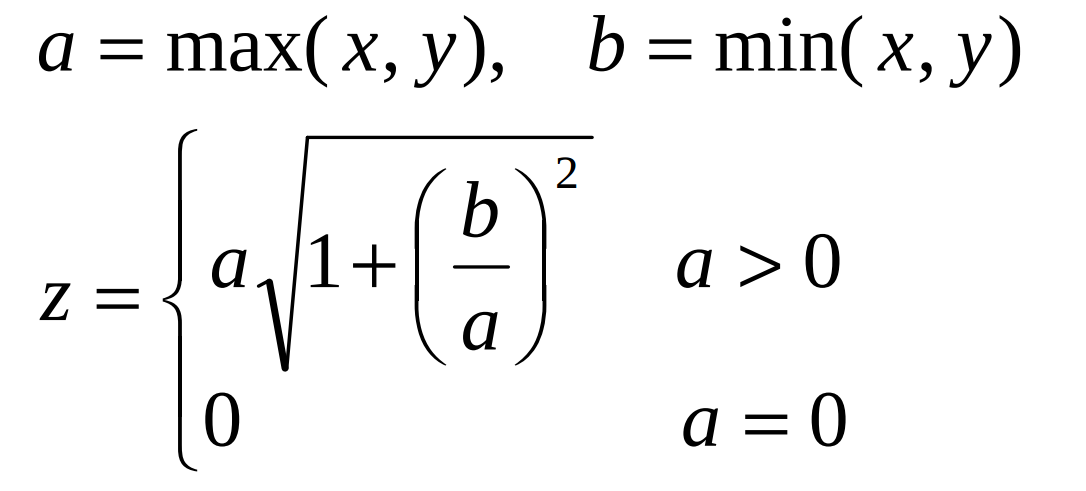
\includegraphics[width=0.3\textwidth]{images/safe-pythag}
\end{center}

\subsection{Condition of a problem}

The condition of a problem is how sensitive it is to changes in the data. A
problem is ill-conditioned if a small change in the data results in a large
change in the solution. This is concerned with the problem, not the method used
to solve it.

Consider the equation $x^3 - 21 x^2 + 120x - 100 = 0$; the solutions are $x =
\{1, 10\}$. However, if we change the value of $x^3$ to $0.99$ or $1.01$, then
the roots become $x = \{1, 11.17, 9.041\}$ and $x = \{1, 9.896 \pm 1.044\}$
respectively.

We can work out the sensitivity by using partial differentiation, if the
perturbed function if $\bar{f}(x) = f(x) + \epsilon g(x)$, where $g(x)$ is the
change applied to $f(x)$, then:

\[
  |\delta| \approx |\frac{\epsilon g(x)}{f'(x)}|~\text{(single root)}
\]

\[
  |\delta| \approx |\sqrt{-\frac{2\epsilon g(x)}{f''(x)}}|~\text{(double root)}
\]

In the above example, $g(x) = x^3, \epsilon = -0.01, f'(x) = 3x^2 - 42x + 120$:

\[
  |\delta| \approx |\frac{-0.01 \times 1^3}{81}| \approx 0.0001
\]

For the double root, $f''(x) = 6x - 42$

\[
  |\delta| \approx |\sqrt{-\frac{2 \times -0.01 \times 1000}{18}}| \approx 1.054
\]

So the double root is vastly affected, but the single root isn't.

\subsection{Stability}

The stability of a method is how sensitive it is to rounding errors. A method
that guarantees as accurate solution as the input data allows is said to be
stable, otherwise it's unstable. Condition is about the sensitivity of the
problem, but stability is about the sensitivity of the method.

Given the quadratic equation $1.6x^2 - 100.1x + 1.251 = 0$, the solution can be
found using the standard formula (in floating point) ($x = \frac{-b \pm\sqrt{b^2
- 4ac}}{2a}$), which gives $x = \{62.53, 0.03125\}$.

If we only compute the first root to be $x_1 = 62.53$, but use $x = c/ax_1$ for
the second, then we get the second root to be $0.01251$. The correct solutions
are $x = \{62.53, 0.0125\}$.

The problem was that $y_1 = -b = 100.1$, and  $y_2 = \sqrt{b^2 - 4ac} = 100.06$.
Since if we do subtraction with very close numbers, the error is high. If we
calculate $\delta$ for this then we get:

\[
  \delta = X(\log_10\frac{|y_1| + |y_2|}{|y_1 - y_2|}) = 4
\]

Meaning all of our digits were rubbish!

%TODO: Page 41 onwards for an example

% Part two of the course!

\section{Optimisation and nature inspired algorithms}

To start, lets recap some stuff you should already know; a minima is a point of
a function where all points in its vicinity have a higher value than itself,and
a maxima is the opposite; a point where all points in its vicinity have a lower
value than itself.

Since we can invert a function by putting a minus in front of it, we don't
really need to differentiate between maxima and minima, since we can always
express on in terms of the other.

Global optimums are the best values for the entire domain, while local optimums
are best in some bounded region.

One dimensional functions are easiest to visualise; they are just a graph, where
the y value is the value of the function and the x value is the input. As the
dimensionality increases, the functions get harder to visualise; 2d functions
are visualised on a 2d graph, where the intensity of the colour in each square
represents the value of the function at that coordinate. 

% TODO: inequality/equality constraints?

An optimisation problem is one where we attempt to maximise or minimise a
function. This involves finding the input that will produce the largest or
smallest value. Optimisation problems are really search problems; given a
domain, find an input that produces the smallest output.

If we know exactly what the function we're trying to optimise is (i.e. we have
an equation), then it's an explicit problem, but if we just have some inputs and
outputs, then it's a black box problem.

Similarly, there are two different approaches to solving these problems:

\begin{description}
  \item \textbf{Single solution}:\\
   This is where there is a single candidate solution that is incrementally 
   improved by the algorithm throughout the procedure.
  \item \textbf{Population based solution}:\\
    This is where there is a set of candidate solutions (the population) and an
    iterative operation combines the best ones to improve the quality of the 
    population.
\end{description}

All of the optimisation methods follow a cycle:

\begin{itemize}
  \item Guess some parameters for the initial solution
  \item While we're not satisfied:
  \begin{itemize}
    \item Evaluate how the current parameters perform
    \item If we're satisfied, then we've finished
    \item Otherwise, then determine new parameters based on the current ones
      and their evaluation.
  \end{itemize}
\end{itemize}

We can use derivatives to try and find maxima and minima in a function. If we do
not have an explicit function for the derivative, then we can calculate them
using \textbf{finite differences}:

\begin{description}
  \item \textit{Forward difference}:\\
    \[
      f'(x) \approx \frac{f(x + h) - f(x)}{h}
    \]
  \item \textit{Central difference}:\\
    \[
      f'(x) \approx \frac{f(x + h) - f(x - h)}{2h}
    \]
\end{description}

Here, the $h$ parameter is the range over which we're calculating the
differential.

\subsection{Minimising univariate functions}

For one dimensional functions, we can use two approaches:

\begin{itemize}
  \item Interval reduction, where we iteratively reduce the range of values that
  we think the optimum is inside.
  \item Interpolation, where we try to find an approximate function and use the
  optimum of that function to iterate to find a better approximate function.
\end{itemize}

\subsubsection{Bisection algorithm}

This is the easiest algorithm, we start with the full range in the domain, and
then cut it in half based on the value of the differential at the midpoint at
the range.

\begin{verbatim}
  bisection(f'(x), a, b, e) {
    while (b - a >= e) {
      c = (a + b) / 2;
      if (f'(c) < 0) a = c;
      else if(f'(c) > 0) b = c
      else return c;
    }
  }
\end{verbatim}

\subsubsection{Quadratic interpolation algorithm}

Here, we make a quadratic function that goes through three points $a, b$ and
$c$, then we either drop $a$ or $b$ depending on which way we should move the
quadratic function. Here, \textbf{we do not need the differential} which is good
since we won't always have it!

% TODO: Insert & explain psudo code

\begin{verbatim}
  Sudo insert psudo code
\end{verbatim}

\subsubsection{Stopping criteria}

Eventually, we will have to stop our optimisation algorithms, but some of them
will run indefinitely. We need criteria to make them stop after a sane amount of
time. The simple approach is to stop after $n$ iterations, and is applicable to
all iterative functions. The more clever approach is to only stop when we reach
a certain threshold, i.e. when a method converges asymptotically on an optimum.

\subsection{Minimisation of multivariate functions}

There are two different classes of minimisation methods for multivariate
functions:

\begin{description}
  \item \textbf{Based on derivatives}:\\
    Moves are determined based on information from derivatives of the 
    multivariate function.

    A \textit{directional derivative} is a derivative indicating the rate of
    change in a specific dimension:

    % TODO: Give an example of this, since it's really quite vague.

    \[
      \Phi'_r = \lim_{h \rightarrow 0}\frac{f(x + hr) - f(x)}{h}
    \]

    Where $r$ is the direction. If $\Phi'_r$ is positive, then the direction is
    ascending, if it's negative, then the direction is descending and if it's
    equal to zero, then there is no slope.

    Finding the gradient of a vector of a multidimensional function $f(x)$ (and
    hence the vector of all partial derivatives) is:

    \[
      \frac{\delta f}{\delta x_j} =
        \lim_{h \rightarrow 0} \frac{f(x + he_j) - f(x)}{h}
    \]

    $e_j$ is the unit vector in the direction of axis $j$, so to construct the 
    whole gradient for the vector, we need to do:

    \[
      \Delta f(x) = \begin{bmatrix}
        \frac{\delta f}{\delta x_1}(x) & \frac{\delta f}{\delta x_2}(x) & \dots,
        \frac{\delta f}{\delta x_n}(x)
      \end{bmatrix}^{T}
    \]

    The \textbf{Hessian} is the matrix containing the second order partial
    derivatives, and is always of size $N \times N$:

    \[
      Hf(x) = \begin{bmatrix}
        \frac{\delta^2 f}{\delta x_1 \delta x_1}(x) & \dots &
          \frac{\delta^2 f}{\delta x_1 \delta x_n}(x)\\
        \vdots & \ddots & \vdots\\
        \frac{\delta^2 f}{\delta x_n \delta x_1}(x) & \dots &
          \frac{\delta^2 f}{\delta x_n \delta x_n}(x)\\
      \end{bmatrix}
    \]

    Most algorithms have some kind of \textit{parameter update scheme}, where
    they will move in a given direction $r$ for a length of $\alpha$ every
    iteration,  and $r, \alpha$ change based on the current position:

    \[
      x_{i+1} = x_i + r_i\alpha_i
    \]

    \subsubsection{The alternating variable method}

    A conceptually easy method, you start from an arbitrary position $x$, and
    then for each dimension $d$:

    \begin{itemize}
      \item Find the differential for that dimension
      \item Find the minimum according to that differential
      \item Move the value of $x_d$ to be equal to that minimum.
    \end{itemize}

    Then repeat for all dimensions until no progress is made.

    %TODO: Insert picture

    \subsubsection{Newton's method}

    As soon as Newton invented calculus, he also started inventing methods for
    finding minima. This method requires a function to be twice differentiable:

    \[
      x_{i+1} = x_i - \alpha\frac{\Delta f(x_i)}{Hf(x_i))}
    \]

    %TODO: Give an example of this...

    The trouble with Newton's method is that it will only converge if the
    initial point is close to the solution, and the memory requirements for the
    Hessian matrix is $n^2$.

  \item \textbf{Direct search}:\\
    Moves are determined using methods other than derivatives, for example,
    using geometric concepts.

    \subsection{Simplex methods}

    If you did Advanced Algorithms 1, you're either groaning now or you're
    jumping for joy at being able to skip a section. However, these aren't the
    simplex methods you learned about last semester.

    For this, you construct a simplex (a shape of $n+1$ vertices in $n$
    dimensions), and then observe that you can always form a new simplex from an
    existing one by adding a new point.

    The \textbf{Spendley, Hext and Himsworth method} is like so:

    \begin{enumerate}
      \item Create $n+1$ vectors for a regular simplex (where all sides are the
      same length).
      \item For each vector, the value of the objected point is calculated for
      that point.
      \item The vector with the highest point is removed and substituted by a 
      new one.
      \item If the worst vector is also the most recently introduced one, then
      the next worst one is used.
      \item The newly substituted vector is the mirror image of the old one
      along the axis of the remaining vectors. %TODO: Equation
      \item When the simplex simply rotates around a point, then
      the vertex in the middle is the minimum.
    \end{enumerate}

    The maximum age of a vector is $1.65n + 0.05 n^2$, and if a vertex exceeds
    age $a$, then the search stops, or is restarted using a smaller simplex.
    If the search was restarted, then the initial (smaller) simplex is started
    from the site of the rotating.

    The \textbf{Nelder and Mead method} is similar, though the simplices are no
    longer regular (though they can be). It involves having rules that either
    expand, contract or reflect the simplex (or any combination of them), which
    leads to quicker results and better approximations of the solution.

    Where $y^{(r)}_0$ is the best value in the previous simplex, and
    $y^{(r)}_{n-1}$ is the worst, the new simplex results from:

    \begin{description}
      \item $y^{(r)}_0 < y^{(r+1)}_{i} < y^{(r)}_{n-1}$:\\
        The simplex is reflected like in the SHH method.
      \item $y^{(r+1)}_{i} < y^{(r)}_{0}$:\\
        The simplex is reflected and expanded.
      \item $y^{(r+1)}_{i} > y^{(r)}_{n-1}$:\\
        The simplex is reflected and contracted.
    \end{description}
\end{description}

% Lecture 3 of part 2

\subsection{Optimisation and nature inspired algorithms}

As we have seen, a global optimum is the best set of admissible conditions to
achieve an objective (i.e. minimising the function) under a set of constraints.

Finding such an optimum is non-trivial, mainly because the search space is often
continuous, so there are an infinite number of parameters to test. The following
algorithms try to find global optimums:

\begin{description}
  \item \textbf{Grid Search}:\\
  We overlay a grid onto the search space (in as many dimensions as we need to),
  and test each point on the grid. We can change the resolution of the grid by
  making the space between the grid lines larger or smaller. The algorithm
  scales exponentially in the number of dimensions, but linearly in the number
  of points tested (dependent on the grid resolution), therefore the runtime is
  $O(n^d)$.

  The quality of the solution depends on the density of the grid, but getting a
  high quality solution is usually impractical, since the search space grows so
  quickly (even in two dimensions, it is quadratic).

  \item \textbf{Random search}:\\
  Here, we simply generate $n$ random points and sample the objective function
  at these points. The point that gives the best value for th objective
  function is remembered for possible later use (since that's the optimum).
  Obviously this algorithm runs in $O(n)$ time, and its quality depends on the
  number of random points chosen. It is possible that the random search method
  could outperform all the other methods if it got lucky, though this is
  unlikely.

  Due to its ease of implementation, random search is often used as a reference
  for other methods.

  \item \textbf{Multistart}:\\

  Here, we guess $n$ random points again, but for each one, we find the local
  minimum. This improves the quality (since there's more chance of finding the
  global minimum, since it's definitely a local minimum too), but it can degrade
  performance.

  This method often visits the same local minima multiple times (if
  optimisations aren't made to avoid doing this) so it can be inefficient.

  \item \textbf{Random walk}:\\
  We can generate a single random start point, but then generate subsequent
  points by choosing a random direction and length for a vector and adding that
  to the current point.

  \item \textbf{Using nature to help minimise}:\\
  If a crystal is being formed, and it cools slowly, then the atoms in the
  crystal will vibrate around until they are in a local minima, which results in
  some cool shapes. We can use techniques to emulate this to find minima in our
  functions.

  Furthermore in genetics, non-optimal genes are `selected out' of the
  population by natural selection and evolution, leading to a genotype that is
  optimum for the environment.

  The remaining algorithms use nature as inspiration:

  \begin{description}
    \item \textbf{Metropolis algorithm}:\\
      This is an algorithm that emulates an ensemble of particles in equilibrium
      at a certain temperature. It uses the Boltzmann probability density
      function:

      \[
        p.d.f = e^{\frac{-E}{k_BT}}
      \]

      To give the probability that a certain particle configuration with an 
      energy $E$ has a certain temperature $T$.

      In nature, perfect crystals are formed by the cooling down from being
      molten very slowly so that the material can reach an equilibrium at each
      temperature. If the cooling is too fast, then an equilibrium will not be
      reached at each temperature, and the crystal will have imperfections.

      Local optimisation algorithms have parallels with letting crystals cool
      too fast!

      The algorithm is as follows:

      \begin{itemize}
        \item Start with a random position for an atom $x^0$
        \item Create a small random displacement to obtain $x^1$ and calculate
        the difference in energy $\Delta E = E^1 - E^0$.
        \item If $\Delta E < 0$ accept the new position, otherwise accept it
        with a probability of $P(\Delta E) = e^{\frac{-\Delta E}{k_BT}}$
        \item Iterate a lot of times, simulating the thermal motion of particles 
        in a heat bath of temperature $T$.
      \end{itemize}

      The Metropolis algorithm works because it lets the energy of the particle
      increase even though that's a `step back' in terms of optimisation.
      Sometimes the algorithm needs to get out of a local minima in order to
      find the global optimum.
    \item \textbf{Simulated Annealing}:\\
      This takes advantage of the fact that we can see the energy of a particle
      was similar to the value of an objective function we're trying to
      maximise, and the coordinates that it is at as similar to the parameters
      of the function we're finding an optimum for.

      The only other variable is the temperature, which acts as a control
      parameter with the same units as the objective function. Simulated
      annealing starts by melting the objective function at a high temperature,
      then using the Metropolis algorithm to calculate the equilibrium of the
      objective function at temperature decreases. Here's the algorithm:

      \begin{itemize}
        \item Start with a high temperature $T^0$ at some random position
        $x^{(0, T^0)}$.
        \item Apply the Metropolis algorithm to determine the average 
        equilibrium value of the objective function and parameter values
        $x^{(Ex, T^0)}$.
        \item keep reducing $T$ and repeating the previous step, and only stop
        when the function freezes; you've reached the global minimum.
      \end{itemize}

      Note that the start position is irrelevant, since there are many
      iterations required for each temperature, and an equilibrium is found for
      each. The start temperature, $T^0$ is very important though; if its too
      low, then a local minimum will be found, and if its too high, then the
      algorithm will take too long.

      \marginpar{Random and grid searches are also asymptotically complete, but
      they converge at much slower rates.}

      Simulated annealing can be reformulated computationally as a Markov Chain,
      and a proof has been given that states the algorithm will converge to a
      global optimum in infinite time, which makes simulated annealing
      \textit{asymptotically complete}.

    \item \textbf{Press' modification}:\\
      In 1989, Press et al. suggested that each temperature cycle should last
      for a predetermined number of iterations $N$. After each cycle, the
      temperature should be reduced by a constant factor $p$:

      \[
        T^{n+1} = pT^n~~~< 0\leq p \leq 1
      \]

      If after a cycle has finished, there have been no successful moves, then
      the algorithm stops. If we increase $N$, then the accuracy increases, but
      the execution time increases faster too. Similarly if we increase $p$, the
      solution will improve (and the reliability too), but the rate of cooling
      drops so it takes longer.

      There is also a slight modification to the displacement step; a single
      parameter is changed to a random value within the boundaries of the
      parameter.

    \item \textbf{Corana's modification}:\\
      Corana et al. suggested that the displacement step should be based off a
      vector; each parameter is changed according to the same coordinate of a
      vector $v_i$. After $N_s$ rounds, $v_i$ is changed so half the new
      candidate parameters are changed. Just like Press' modification, after
      $N_r$ rounds, the temperature is reduced.

      As a result, the annealing will adapt to the shape of the function, but
      it is also slower; $N$ in Press' algorithm is equal to $N_s \times N_r$ in
      Corana's algorithm.
  \end{description}

\end{description}

% Lecture 4 of part 2

\subsection{Evolutionary algorithms}

Natural populations evolve by having variation amongst the members of the
population and having selection (or unfit members of the population dying before
they get chance to reproduce). Evolutionary algorithms are a class of
optimisation algorithms that evolve candidate solutions as a group (ensemble)
rather than looking at one solution at a time.

If you took a biology course at some point, then you may be able to figure this
out, but there is a mapping from biology terminology to CS terminology:

\begin{itemize}
  \item Gene  - Parameter
  \item Chromosome - All parameters
  \item Individual - Candidate solution
  \item Generation - One iteration
  \item Fitness - Value of the objective function
\end{itemize}

Evolutionary algorithms evolve their populations. This means there will be $n$
points in the parameter space, and each iteration will drop some of the points
and create new ones (hopefully, in better locations). Each individual in the 
population is a single candidate solution, and is stored as a
\textit{chromosome}. This is a sequence of bits, split into $m$ sections called
\textit{genes}. As described above, each gene maps onto a parameter.

% TODO: Insert image showing chromosome/genes = parameters

Fogel's algorithm for evolutionary programming is as such:

\begin{enumerate}
  \item Generate a random initial population of $n$ individuals
  \item Calculate the fitness of each individual in the population (using the
  objective function)
  \item Each individual from the current population generates and offspring by
  copying its own genes
  \item Mutate each gene for each chromosome in the offspring by a small 
  variance.
  \item Put the offspring in a new population, $2n$ large
  \item Probabilistically select $n$ individuals as a function of fitness to be
  removed (now we have a population of $n$ again).
  \item Go back to step 2, or stop.
\end{enumerate}

% TODO: Can this be a negative number?

In this algorithm, we described mutation (in step 4) and selection (in step 6).
For mutation, we add a small random number to the original value of a gene.

For selection, we want to select $n$ individuals, where better individuals have
a greater chance of remaining in the population. A roulette wheel is a manual
way of doing this, but stochastic ranking (e.g. a sort that has a chance of
being wrong) or a tournament where each individual is compared against a small
number of others and receives a score based off of its performance; the $n$
lowest scoring individuals are pruned.

Holland and DeJong's Genetic algorithm is as follows. It encodes parameters in
binary, and genes are therefore strings of binary digits.

\begin{enumerate}
  \item Generate $n$ random individuals for the population
  \item Calculate the fitness of each individual in the population
  \item Choose two parent individuals from the current population as a 
  probability of their fitness
  \item Cross them over (see below) at a random locus to produce two offspring
  \item Mutate each locus (gene) in the offspring with a small probability
  \item Put the offspring in the new population
  \item Go to step two, or stop.
\end{enumerate}

The mutation operation flips bits in a gene with a small probability. The cross
over operator swaps the latter halves of two chromosomes at a random index.

% TODO: Cross over image

The differences in the two algorithms are as follows:

\begin{center}
  \begin{tabularx}{0.8\textwidth}{X|X}
    \textbf{Evolutionary programming} & \textbf{Genetic algorithms}\\ \hline
    Genes are encoded as floating point numbers & Genes are encoded in binary.\\
    Mutation is addition of a random value & Mutation is bit flipping.\\
    Asexual reproduction (two parent makes one child) & Sexual reproduction (two
    parents make two children.)\\
    No cross over & Cross over by swapping subsections of the chromosome.
  \end{tabularx}
\end{center}

%TODO: What is the standard deviation gene?
Rechenberger and Schwefel made another algorithm:

\begin{enumerate}
  \item Generate $n$ random individuals
  \item Calculate the fitness of each
  \item Randomly pair up individuals
  \item Recombine them to create two offspring
  \item Mutate each gene locus with a small probability
  \item Put the offspring in the new population ($2n$ large)
  \item Select the best $n$
  \item Go back to step 2, or stop.
\end{enumerate}

% TODO: How is std. deviation incorperated in mutation & recombination

I should figure out how std. deviation incorporates in here...

It is important to note the differences between selection and variation so we
can get the balance right:

\begin{itemize}
  \item Selection is responsible for keeping improvements in the population and
  not discarding them
  \item Very strong selection limits the variation and all individuals will be 
  the same
  \item Mutation and cross over are responsible for introducing variation and 
  will make the parameters/gene pool change
  \item Very strong variation results in good solutions, but they will be 
  replaced by random ones and not retained.
\end{itemize}

Many genetic algorithms progress at very slow rates, but then have short bursts
of very rapid progress. In general, it is not common for these algorithms to
have proven convergence properties, but some of them do when applied to simple
problems.

%TODO: Split this uber sentence up

Deciding when to stop a genetic algorithm isn't always simple; stopping after a
predetermined number of generations requires lots of trial and error to get the
number right, waiting until a desired fitness is reached is okay if you know
what the optimal fitness is, but it may take an (infinitely) long amount of
time, and waiting for the fitness variations from one population to the next to
become stable isn't a good idea either because of the propensity for genetic
algorithms to progress very slowly then have a burst of progress.

% Part 2 Lecture 5

\subsubsection{Genetic programming}

Most evolutionary algorithms try and optimise the parameters of a
function to find a minima, however, genetic programming aims to change
the function until it fits our purpose. If we view computer programs
as mathematical functions (which they are at some level), then we can
evolve computer programs in this way.

Genetic programming evolves programs in two ways; generating new
sections of code and combining or mutating existing code. This
analogous to how a programmer works if you think about it!

If you've taken the compilers course, you're most likely already
comfortable with representing programs as trees. We can represent a
program as a tree with nodes that are either \textit{functions} or
\textit{terminals}. Terminals are either inputs, constants or
programming statements without arguments, while functions are
programming statements, arithmetic functions or operations.

In order to generate a program using genetic programming, you must
define both a function set and a terminal set. These are the sets of
allowable nodes that you can have in your program tree. Examples
include \texttt{XOR}, \texttt{READ}, \texttt{IF} etc for functions and
named variables, random variables or constants for the terminals.

% TODO: Insert a figure of a tree, preferable a side figure so it
% doesn't interrupt the flow?

Of course, every program tree must be semantically correct; function
nodes should have the correct amount of children (one for each
argument), they must be of the correct type. Furthermore, since we're
aiming to generate these trees automatically, we need to account for
when things go wrong. What if we pass $-1$ into a logarithmic
function? We can either make functions that fail return a default
value, or have them throw exceptions that reduce the overall program
fitness.

Cramer and Koza made the following genetic programming algorithm:

\begin{enumerate}
  \item Initialise a random population of $n$ individuals.
  \item Calculate the fitness of each individual in the population
    (i.e. how well the function represented by each individual
    performs).
  \item Select two parents at random proportionally to their fitness
    and reproduce them, producing new children.
  \item Apply cross-over and mutation with a certain probability.
  \item Remove all the parents.
  \item Go back to step 2 unless satisfied.
\end{enumerate}

Unfortunately, we're not finished yet. We need to have some checks on
our trees to make sure that they don't become too large. First of all,
we need to make sure that we generate sensible trees. We can do this
in two ways:

\begin{description}
  \item \textbf{Full method}:
    \begin{itemize}
      \item Choose a random function node.
      \item If the maximum depth has been reached, then fill the child
        nodes with terminals.
      \item Otherwise, recurse for the child nodes of the function.
    \end{itemize}
  \item \textbf{Grow method}:
    \begin{itemize}
      \item Choose a function or a terminal node at random.
      \item If the maximum depth has been reached, then fill the child
        nodes with terminals.
      \item Otherwise, recurse for the child nodes of the function.
    \end{itemize}
\end{description}

Essentially, the \textit{full} method generates trees that are always
of a specific depth (and each subtree of every node is of the same
depth, unless you allow nodes with no arguments in your functions
set). The \textit{grow} method will give you a larger range of trees,
some will be far smaller than those generated by the other method (a
terminal node could be picked on the first iteration for example).

Mutation is applied to single individuals, where a node is chosen at
random, and replaced by a randomly generated sub-tree. The sub-tree
could be the same depth as the removed node if you wanted to preserve
the depth of the tree (though sometimes deeper, more complicated
functions may be needed to encapsulate the intricacies of the
reference function).
